\documentclass[aps,prl,reprint,superscriptaddress,nofootinbib]{revtex4-2}

\usepackage[T1]{fontenc}
\usepackage{amsmath,amssymb,amsthm,mathtools,bm}
\usepackage{newtxtext,newtxmath}
\usepackage{microtype}
\usepackage{balance}
\usepackage{tikz}
\usetikzlibrary{arrows.meta,fit,positioning}
\usepackage[colorlinks=true,allcolors=blue]{hyperref}

\allowdisplaybreaks

\newcommand{\M}{\mathrm{M}}
\newcommand{\I}{\mathrm{I}}
\newcommand{\C}{\mathbb C}
\newcommand{\id}{\operatorname{id}}
\newcommand{\Ad}{\operatorname{Ad}}
\newcommand{\Tr}{\operatorname{Tr}}
\newcommand{\PPT}{\operatorname{PPT}}
\newcommand{\EB}{\operatorname{EB}}
\newcommand{\CP}{\operatorname{CP}}
\newcommand{\Pos}{\operatorname{Pos}}
\newcommand{\SEP}{\operatorname{SEP}}
\newcommand{\Sym}{\operatorname{Sym}}
\newcommand{\supp}{\operatorname{supp}}
\newcommand{\vecop}{\operatorname{vec}}
\newcommand{\cB}{\mathcal B}
\newcommand{\cS}{\mathcal S}
\newcommand{\cU}{\mathcal U}
\newcommand{\Tmap}{\mathsf T}

\newtheorem{theorem}{Theorem}
\newtheorem{lemma}[theorem]{Lemma}
\newtheorem{proposition}[theorem]{Proposition}
\newtheorem{corollary}[theorem]{Corollary}
\newcommand{\suppsection}[2]{%
 \refstepcounter{section}%
 \section*{\thesection.\ #1}%
 \label{sm:#2}}

\begin{document}

\title{PPT Map Composition Is Entanglement Breaking When One Dimension Is Two}
\author{Ao-Xiang Liu}
\affiliation{School of Physical Sciences, University of Chinese Academy of Sciences, 1 Yanqihu East Rd, Beijing 101408, China}
\date{August 18, 2026}

\begin{abstract}
The positive partial transpose (PPT) squared conjecture asks whether applying a
completely positive and completely copositive map twice must produce an
entanglement-breaking map.  We prove its equivalent two-map formulation
whenever the input, intermediate, or output matrix algebra is $\M_2$, with the
other dimensions arbitrary and independent.  In the state formulation, we
also prove that every postselected measurement outcome on the intermediate
systems of two PPT states is separable across the end systems if any one of
the four local systems is a qubit.  We also show that the composition of any
two composable PPT maps is 2-entanglement breaking, as is its adjoint.
Schmidt-number iteration then gives a uniform bound: any $2(d-1)$ PPT maps on
$\M_d$ compose to an entanglement-breaking map.
\end{abstract}

\maketitle

\textit{Introduction.---}
Quantum channels are composed whenever a noisy process is used repeatedly or
several elementary links are connected in a network.  Entanglement-breaking
maps mark the point at which a channel can no longer transmit entanglement:
acting on one part of any bipartite state always produces a separable
operator~\cite{Horodecki2003}.  Positive partial transpose (PPT) maps form a
larger class.  Their Choi operators have positive partial transpose but may
still be entangled, just as PPT states may contain bound entanglement
\cite{Horodecki1998}.  Determining when PPT maps become entanglement breaking
under composition therefore probes how repeated noise erases quantum
correlations and whether one-shot entanglement swapping can entangle the end
systems of two PPT links in a repeater network
\cite{Briegel1998,Bauml2015}.

The PPT squared conjecture asks what happens after two successive maps
\cite{Christandl2019}.  Its original form asks whether $T\circ T$ is
entanglement breaking for every PPT map $T:\M_d\to\M_d$, without assuming
trace preservation.  Christandl, M\"uller-Hermes, and Wolf proved that this
is equivalent to the corresponding statement for two possibly different
composable PPT maps $T_1:\M_{d_0}\to\M_{d_1}$ and
$T_2:\M_{d_1}\to\M_{d_2}$.  The Choi--Jamiołkowski correspondence relates
this formulation to entanglement swapping.  Placing the two Choi operators on
adjacent links and projecting their intermediate systems onto the standard
maximally entangled state produces the Choi operator of $T_2\circ T_1$
\cite{Singh2022,An2026}.  This identifies map composition with the standard
maximally entangled postselection in a single entanglement-swapping step and
raises the broader question whether an arbitrary postselected measurement can
entangle the end systems of two PPT links.

Two lines of work describe the progress toward this question.  For repeated
applications of one channel, entanglement-breaking indices quantify the
number of uses required to destroy all entanglement~\cite{Lami2015}.
Kennedy, Manor, and Paulsen proved asymptotic convergence to the
cone of entanglement-breaking maps for unital or trace-preserving PPT maps
\cite{Kennedy2018}.  Finite indices were then established for unital PPT maps
and for PPT maps whose Perron eigenmatrices have full support
\cite{Rahaman2018,Hanson2020}.  Park recently proved that every PPT map has
finite entanglement-breaking index and asked whether the index admits a bound
depending only on the dimension~\cite{Park2026}.

For the two-map formulation on $\M_d$, the conjecture is immediate for $d=2$
and was proved for $d=3$ by Christandl,
M\"uller-Hermes, and Wolf and independently by Chen, Yang, and Tang
\cite{Horodecki1996,Christandl2019,Chen2019}.  Further results cover Gaussian
channels, Choi-type maps, and stronger qutrit composition statements
\cite{Christandl2019,Singh2022,An2026}.  Henry very recently proved the case
$\M_{d_0}\to\M_2\to\M_{d_2}$ for arbitrary $d_0$ and $d_2$
\cite{Henry2026}.

In this work, we prove that $T_2\circ T_1$ is entanglement breaking whenever
any one of $d_0,d_1,d_2$ equals two, with no relation required between the
other dimensions.  We establish $d_2=2$ using an auxiliary operator with a
qutrit factor and a normal form for positive maps with two-dimensional
domain, and obtain $d_0=2$ by Hilbert--Schmidt adjunction.  A separate
argument in the Pauli representation gives an independent proof of the case
$d_1=2$.  We further prove that every postselected outcome of two PPT links is
separable across the end systems whenever any one of the four local systems
is a qubit, even when the measured dimensions differ.

The proof for $d_2=2$ also implies that both the composition of any two PPT
maps and its adjoint are 2-entanglement breaking.  Schmidt-number iteration
then shows that any $2(d-1)$ PPT maps on $\M_d$, not necessarily identical,
compose to an entanglement-breaking map.  In particular,
$n_{\rm EB}(T)\leq2(d-1)$ for every PPT map $T:\M_d\to\M_d$, answering
Question~4.3 of Ref.~\cite{Park2026}.

\begin{figure}[t]
\centering
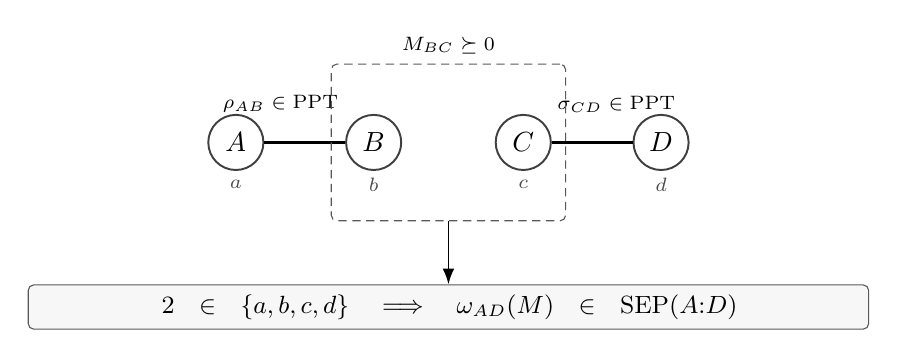
\begin{tikzpicture}[
  site/.style={circle,draw=black!75,fill=white,line width=0.7pt,
    minimum size=7mm,inner sep=0pt},
  link/.style={line width=0.8pt},
  dim/.style={font=\scriptsize,text=black!70},
  relay/.style={draw=black!65,densely dashed,rounded corners=2pt,
    inner xsep=5pt,inner ysep=18pt},
  result/.style={draw=black!65,fill=black!3,rounded corners=2pt,
    align=center,text width=0.86\columnwidth,inner sep=3.5pt,font=\small}
]
\node[site] (A) at (0,0) {$A$};
\node[site] (B) at (1.75,0) {$B$};
\node[site] (C) at (3.65,0) {$C$};
\node[site] (D) at (5.40,0) {$D$};
\draw[link] (A)--node[pos=0.20,above=7pt,font=\scriptsize]
  {$\rho_{AB}\in\PPT$} (B);
\draw[link] (C)--node[pos=0.80,above=7pt,font=\scriptsize]
  {$\sigma_{CD}\in\PPT$} (D);
\node[dim] at ([yshift=-5pt]A.south) {$a$};
\node[dim] at ([yshift=-5pt]B.south) {$b$};
\node[dim] at ([yshift=-5pt]C.south) {$c$};
\node[dim] at ([yshift=-5pt]D.south) {$d$};
\node[relay,fit=(B)(C),label={[font=\scriptsize]above:$M_{BC}\succeq0$}]
  (relay) {};
\node[result,below=8mm of relay] (result)
  {$2\in\{a,b,c,d\}\ \Longrightarrow\
    \omega_{AD}(M)\in\SEP(A{:}D)$};
\draw[-{Latex[length=2mm]},line width=0.65pt]
  (relay.south)--(result.north);
\end{tikzpicture}
\caption{One-shot entanglement swapping between two PPT states.  For arbitrary
local dimensions and any positive measurement operator $M_{BC}$ on the
intermediate systems, the unnormalized operator on $A{:}D$ is separable if
$2\in\{a,b,c,d\}$.  The operator $M_{BC}$ need not be rank one or
projective, and $b$ and $c$ need not be equal.}
\label{fig:swapping}
\end{figure}

\textit{Main result.---}
For a map $\Phi$, use the Choi operator
\begin{equation}
 J_\Phi=\sum_{i,j}E_{ij}\otimes\Phi(E_{ij}),
\label{eq:choi}
\end{equation}
with partial transpose on the second factor.  A map is PPT when its Choi
operator is positive and PPT, and entanglement breaking (EB) when its Choi
operator is separable~\cite{Choi1975,Horodecki2003}.  No map below is assumed
trace preserving, unital, invertible, or of fixed rank.

\begin{theorem}
\label{thm:anywhere}
Let
\begin{equation}
 \Phi_1:\M_{d_0}\longrightarrow\M_{d_1},\qquad
 \Phi_2:\M_{d_1}\longrightarrow\M_{d_2}
\label{eq:pair}
\end{equation}
be PPT maps.  If $2\in\{d_0,d_1,d_2\}$, then
$\Phi_2\circ\Phi_1$ is entanglement breaking.  The other two dimensions
are arbitrary and independent.
\end{theorem}

The proof has two branches.  We establish $d_2=2$ directly and obtain
$d_0=2$ by adjunction; an independent Pauli argument proves $d_1=2$.

\textit{Composition with a two-dimensional output algebra.---}
When the output algebra is $\M_2$, the adjacent $2\otimes d$ PPT Choi
operator may itself be entangled.  Separability of the composed Choi operator
is instead equivalent to the following bilinear positivity statement.  Here
$\PPT(n,d)$ denotes the cone of positive operators on
$\C^n\otimes\C^d$ whose partial transpose on the second factor is positive.

\begin{lemma}
\label{thm:bilinear}
For all $n,d\geq1$, every positive map $T:\M_2\to\M_d$, every
$X\in\PPT(n,d)$, and every $R\in\PPT(n,2)$,
\begin{equation}
 \Tr\!\left[X(\id_n\otimes T)(R)\right]\geq0\,.
\label{eq:bilinear}
\end{equation}
\end{lemma}

The quantifier over all positive $T$ is essential: their Choi operators form
the cone of block-positive operators.  The proof constructs an operator $Q$
with a qutrit factor
from $R$ and then reduces every such $T$ to positive maps whose restrictions
to the relevant two-dimensional subspaces are decomposable.

\begin{lemma}
\label{lem:auxiliaryQ}
For every $R\in\PPT(n,2)$, there exists a positive operator
$Q\in\M_n\otimes\M_3$ satisfying
$Q^{\Gamma_{\mathrm{qutrit}}}=Q$, where the superscript transposes the
qutrit factor.  It obeys
\begin{equation}
 (\id_n\otimes\Ad_V)(Q)=R,\qquad
 V=\begin{pmatrix}1&-i&0\\0&0&1\end{pmatrix},
\label{eq:recovery}
\end{equation}
where $\Ad_L(Z)=LZL^*$.  The operator $Q$ also has a pure-state decomposition
in which every vector has Schmidt rank at
most two and its Schmidt vectors on $\C^3$ lie in a conjugation-invariant
subspace of dimension at most two.
\end{lemma}

The operator $Q$ can be constructed explicitly.  Writing $R$ as a
$2\times2$ matrix of blocks in $\M_n$,
$R=\left(\begin{smallmatrix}A&C\\C^*&B\end{smallmatrix}\right)$, with
$C=X+iY$, $X=X^*$, and $Y=Y^*$, determines
\begin{equation}
 \begin{aligned}
 G&=B^+,& \Delta&=A-XGX-YGY,\\[-1mm]
 W&=YGX-XGY,& \Xi&=XGY+YGX.
 \end{aligned}
\label{eq:auxiliaryblocks}
\end{equation}
For $P_B=\supp B$, generalized Schur complements give
$X=P_BXP_B$, $Y=P_BYP_B$, and $\Delta\pm iW\succeq0$.  Define
$\widetilde Q\in\M_3\otimes\M_n$ by
\begin{equation}
 \widetilde Q=
 \begin{pmatrix}
  XGX+\Delta/2&-\Xi/2&X\\
  -\Xi/2&YGY+\Delta/2&-Y\\
  X&-Y&B
 \end{pmatrix},\qquad
 Q=F_{3,n}\widetilde QF_{3,n}^*,
\label{eq:auxiliaryQ}
\end{equation}
where $F_{3,n}$ flips the tensor factors.  Direct multiplication gives
Eq.~\eqref{eq:recovery}, and symmetry of the $3\times3$ block matrix gives
$Q^{\Gamma_{\mathrm{qutrit}}}=Q$.  The operator $\widetilde Q$ has the
positive splitting
\begin{align}
 \widetilde Q&=Q_0+Q_{12},
\nonumber\\[-1mm]
 Q_0&=\begin{pmatrix}X\\-Y\\B\end{pmatrix}
 G\begin{pmatrix}X&-Y&B\end{pmatrix},
\nonumber\\
 Q_{12}&=\frac12\begin{pmatrix}
  \Delta&-W&0\\ W&\Delta&0\\0&0&0
 \end{pmatrix}.
\label{eq:Qsplit}
\end{align}
For $v_\pm=(e_0\pm i e_1)/\sqrt2$,
\begin{equation}
 Q_{12}=\frac12\left[
 |v_+\rangle\langle v_+|\otimes(\Delta-iW)
 +|v_-\rangle\langle v_-|\otimes(\Delta+iW)
 \right]\succeq0,
\label{eq:Q12decomp}
\end{equation}
and its pure components lie in the subspace
$\operatorname{span}\{e_0,e_1\}$.  The first term in
Eq.~\eqref{eq:Qsplit} is a Gram operator.  On $\supp B$, put
$S=B^{1/2}$, $D=B^{+/2}XB^{+/2}$, and
$F=B^{+/2}YB^{+/2}$.  Diagonalizing the Hermitian matrix
$De_j=d_je_j$ gives, after the tensor flip, Gram vectors
\begin{equation}
 |\xi_j\rangle=Se_j\otimes(d_je_0+e_2)-SFe_j\otimes e_1,
 \qquad d_j\in\mathbb R.
\label{eq:qutritsubspace}
\end{equation}
Their Schmidt vectors on $\C^3$ lie in the conjugation-invariant subspace
$\operatorname{span}\{d_je_0+e_2,e_1\}$.  Thus both terms in
Eq.~\eqref{eq:Qsplit} are positive and have the decomposition stated in
Lemma~\ref{lem:auxiliaryQ}.  The treatment of singular $B$ is given
in Ref.~\cite{Supplement}.

This restriction implies the required nonnegative pairing.  If a positive map
$\Lambda:\M_3\to\M_k$ satisfies $\Lambda=\Lambda\circ\Sym$, with
$\Sym(Z)=(Z+Z^{\mathsf T})/2$, then every real isometry
$U:\C^2\to\C^3$ obeys
$\Lambda\circ\Ad_U=(\Lambda\circ\Ad_U)\circ\Tmap_2$.  The restriction is
therefore decomposable, by separability of positive $2\otimes k$ operators
fixed by qubit partial transpose~\cite[Theorem~2]{Kraus2000} and
duality between the PPT cone and decomposable witnesses
\cite{Skowronek2009}.  To apply this fact
termwise, write the decomposition from Lemma~\ref{lem:auxiliaryQ} as
$Q=\sum_\alpha|\psi_\alpha\rangle\langle\psi_\alpha|$.  For each component,
choose a real isometry $U_\alpha:\C^2\to\C^3$ whose range contains its
Schmidt vectors on $\C^3$ and a map $C_\alpha:\C^n\to\C^2$ such that
\begin{align}
 |\psi_\alpha\rangle
 &=\left(\I_n\otimes U_\alpha\right)\vecop(C_\alpha),
\nonumber\\
 (\id_n\otimes\Lambda)
 (|\psi_\alpha\rangle\langle\psi_\alpha|)
 &=J_{(\Lambda\circ\Ad_{U_\alpha})\circ\Ad_{C_\alpha}}.
\label{eq:componentchoi}
\end{align}
Decomposable maps remain decomposable under CP precomposition; for the
copositive part this follows from
$\Tmap_2\circ\Ad_{C_\alpha}
=\Ad_{\overline{C_\alpha}}\circ\Tmap_n$.  Hence every term in
Eq.~\eqref{eq:componentchoi} pairs nonnegatively with a PPT operator, and
\begin{equation}
 \Tr\!\left[P(\id_n\otimes\Lambda)(Q)\right]\geq0
 \qquad\text{for every }P\in\PPT(n,k).
\label{eq:nonnegativepairing}
\end{equation}

We now reduce an arbitrary positive $T:\M_2\to\M_d$ to the map $\Lambda$
and CP maps to which Eq.~\eqref{eq:nonnegativepairing} applies.  Denote the left-hand side of
Eq.~\eqref{eq:bilinear} by
$\cB_T(X,R)$.  The zero map is trivial.  For $T\neq0$, first restrict its
codomain to the support of $T(\I_2)$, which contains the range of every output.
The pairing and the PPT constraints are invariant under invertible input and
output congruences.  Moving a pure input with nonzero output to $e_0$,
whitening that output on its range, and applying an upper shear gives the
following block form.  If the chosen output has rank $k$ and $m=d-k$, then
\begin{equation}
 \begin{aligned}
 T(E_{00})&=\begin{pmatrix}\I_k&0\\0&0_m\end{pmatrix},&
 T(E_{01})&=\begin{pmatrix}H&A\\B^*&0\end{pmatrix},\\[-1mm]
 T(E_{11})&=\begin{pmatrix}C&0\\0&\I_m\end{pmatrix}.
 \end{aligned}
\label{eq:normalizedblocks}
\end{equation}
When $m=0$, the lower blocks are absent.  The restriction to
$\supp T(\I_2)$, the exclusion of common kernel vectors, and the treatment of
singular blocks are given in Ref.~\cite{Supplement}.  From here on, $A,B,C$
denote the blocks in Eq.~\eqref{eq:normalizedblocks}, not the blocks defining
$Q$ above.
For a real vector $x=(u,v,r)^{\mathsf T}$, set
\begin{align}
 M(u,v)&=u(A+B)+iv(B-A),
\nonumber\\
 \cS(x)&=(u^2+v^2)\I_k-M(u,v)M(u,v)^*
\nonumber\\[-1mm]
 &\quad+r\left[u(H+H^*)+iv(H^*-H)\right]+r^2C.
\label{eq:schurform}
\end{align}
Since $Vx=(u-iv,r)^{\mathsf T}$, Eq.~\eqref{eq:normalizedblocks} gives
\begin{equation}
 T((Vx)(Vx)^*)=
 \begin{pmatrix}
  \cS(x)+M(u,v)M(u,v)^*&rM(u,v)\\
  rM(u,v)^*&r^2\I_m
 \end{pmatrix}\succeq0.
\label{eq:pureoutputnormal}
\end{equation}
For $m>0$ and $r\neq0$, the lower-right Schur complement gives
$\cS(x)\succeq0$; continuity covers $r=0$.  For $m=0$, the rectangular
blocks and $M(u,v)$ are absent and the same conclusion follows directly.

Real polarization of $\cS$, followed by complexification and composition
with $\Sym$, defines a complex-linear map $\Lambda:\M_3\to\M_k$ satisfying
\begin{equation}
 \Lambda(xx^{\mathsf T})=\cS(x),\qquad
 \Lambda=\Lambda\circ\Sym.
\label{eq:Lambda}
\end{equation}
This map is positive: if $Z\succeq0$, then
$\Sym(Z)=(Z+\bar Z)/2$ is a real positive matrix and hence a sum
$\sum_\ell x_\ell x_\ell^{\mathsf T}$ with $x_\ell\in\mathbb R^3$;
Eq.~\eqref{eq:Lambda} gives
$\Lambda(Z)=\sum_\ell\cS(x_\ell)\succeq0$.

Let $E:\C^k\hookrightarrow\C^d$ be the canonical inclusion into the first
$k$ coordinates.  For
the standard basis $e_a$ of $\C^m$ and $a=1,\ldots,m$, define
\begin{equation}
 K_a=\begin{pmatrix}
  (A+B)e_a&i(B-A)e_a&0\\
  0&0&e_a
 \end{pmatrix}:\C^3\to\C^d.
\label{eq:Ka}
\end{equation}
Then, abbreviating $M=M(u,v)$,
\begin{align}
 K_ax&=\begin{pmatrix}Me_a\\re_a\end{pmatrix},
\nonumber\\[-1mm]
 \sum_{a=1}^m(K_ax)(K_ax)^*
 &=\begin{pmatrix}MM^*&rM\\rM^*&r^2\I_m\end{pmatrix}.
\label{eq:gramresidual}
\end{align}
For $m=0$ the family is absent.  Adding
$\Ad_E(\Lambda(xx^{\mathsf T}))$ to Eq.~\eqref{eq:gramresidual} reproduces
Eq.~\eqref{eq:pureoutputnormal} for every real $x$; polarization therefore
gives the exact map identity
\begin{equation}
 T\circ\Ad_V\circ\Sym
 =\Ad_E\circ\Lambda+
  \sum_{a=1}^{m}\Ad_{K_a}\circ\Sym.
\label{eq:mapidentity}
\end{equation}
The treatment of the support of $T(\I_2)$ is given in
Ref.~\cite{Supplement}.
Since
$Q^{\Gamma_{\mathrm{qutrit}}}=Q$, inserting Eq.~\eqref{eq:mapidentity} into
Eq.~\eqref{eq:bilinear} yields the identity
\begin{equation}
\begin{aligned}
 \Tr\!\left[X(\id_n\otimes T)(R)\right]
 &=\Tr\!\left[(\id_n\otimes\Ad_{E^*})(X)
        (\id_n\otimes\Lambda)(Q)\right]
 \\[-1mm]
 &\quad+\sum_a\Tr\!\left[(\id_n\otimes\Ad_{K_a^*})(X)Q\right]\geq0.
\end{aligned}
\label{eq:split}
\end{equation}
The first compressed operator is PPT, while every operator in the sum is
positive; Eq.~\eqref{eq:nonnegativepairing} proves Lemma~\ref{thm:bilinear}.

The bilinear inequality proves the case of a two-dimensional output algebra.
For PPT maps
$\Phi:\M_d\to\M_n$ and $\Psi:\M_n\to\M_2$,
adjunction preserves PPT, and therefore $X=J_{\Phi^*}\in\PPT(n,d)$ and
$R=J_\Psi\in\PPT(n,2)$.  A matrix-unit contraction gives
\begin{align}
 \cB_T(J_{\Phi^*},J_\Psi)
 &=\Tr_{\rm HS}(T\circ\Psi\circ\Phi)
\nonumber\\
 &=\Tr\!\left[J_{T^*}J_{\Psi\circ\Phi}\right],
\label{eq:choipairing}
\end{align}
where $\Tr_{\rm HS}S=\sum_{i,j}\Tr[E_{ji}S(E_{ij})]$.  As
$T:\M_2\to\M_d$ ranges over all positive maps, $J_{T^*}$ exhausts the
cone of block-positive operators.  Lemma~\ref{thm:bilinear} makes
Eq.~\eqref{eq:choipairing} nonnegative for every such operator.  Duality
between the cone of block-positive operators and the cone of separable
operators~\cite{Horodecki1996} then makes
$J_{\Psi\circ\Phi}$ separable.  Hence $\Psi\circ\Phi$ is EB.  Applying the
same argument to the adjoint PPT pair proves the case of a two-dimensional
input algebra.

\textit{Two-dimensional intermediate algebra.---}
Very recently, Henry proved the case with a two-dimensional intermediate
algebra using normalized $2\times2$ Choi blocks and operator
interpolation~\cite{Henry2026}.  We give an independent proof using qubit spin
flip and the following separability identity.

\begin{lemma}
\label{lem:rowgram}
For Hermitian $X_j\in\M_a$ and $Y_j\in\M_c$, if
\begin{equation}
 \sum_jX_j^2\preceq\I_a,\qquad
 \sum_jY_j^2\preceq\I_c,
\label{eq:rowbounds}
\end{equation}
then $\I_a\otimes\I_c+\sum_jX_j\otimes Y_j$ is separable.
\end{lemma}

The explicit decomposition into positive product operators is given
in Ref.~\cite{Supplement}.

For $d_1=2$, set $\Psi=\Phi_1^*$ and
$\Theta=\Phi_2$, and whiten them on their output supports to unital PPT maps
$\widehat\Psi$ and $\widehat\Theta$.  Define
$X_j=\widehat\Psi(\sigma_j)$ and
$Y_j=\widehat\Theta(\sigma_j)$ for the three Pauli matrices.  Complete
positivity, complete copositivity, and the qubit
spin flip give
\begin{equation}
 -\I\preceq\sum_j\sigma_j^{\mathsf T}\otimes X_j\preceq\I.
\label{eq:spinflip}
\end{equation}
Functional calculus followed by the normalized qubit trace yields
$\sum_jX_j^2\preceq\I$; the same holds for the $Y_j$.  Hence
\begin{equation}
 J_{\widehat\Theta\circ\widehat\Psi^*}
 =\tfrac12\left(\I\otimes\I+
   \sum_{j=1}^3X_j^{\mathsf T}\otimes Y_j\right)
\label{eq:middlechoi}
\end{equation}
is separable by Lemma~\ref{lem:rowgram}.  Local CP congruences undo the
whitening and preserve separability, proving the case $d_1=2$.  Singular
support details are given in Ref.~\cite{Supplement}.  Together with the input
and output cases above, this completes the proof of
Theorem~\ref{thm:anywhere}.

\textit{Entanglement swapping and consequences for composition.---}
The map theorem has a direct consequence for states.  For the two PPT states
in Fig.~\ref{fig:swapping}, a positive measurement
operator $M_{BC}\succeq0$ on the intermediate systems produces the
unnormalized operator on the end systems
\begin{equation}
\omega_{AD}(M)=\Tr_{BC}\!\left[(\rho_{AB}\otimes\sigma_{CD})
 (\I_A\otimes M_{BC}\otimes\I_D)\right].
\label{eq:swapping}
\end{equation}

\begin{corollary}
\label{cor:swapping}
Let $\dim A=a$, $\dim B=b$, $\dim C=c$, and $\dim D=d$, with no
equality required among these dimensions.  If
$\rho_{AB}\in\PPT(A:B)$, $\sigma_{CD}\in\PPT(C:D)$, and
$2\in\{a,b,c,d\}$, then
\begin{equation}
 \omega_{AD}(M)\in\SEP(A:D)\qquad\text{for every }M_{BC}\succeq0.
\label{eq:selective}
\end{equation}
\end{corollary}

For unequal intermediate dimensions, a rank-one vector can be represented
in two ways using rectangular matrices,
\begin{equation}
 |\eta\rangle=(L_B\otimes\I_C)|\Omega_c\rangle
 =\left(\I_B\otimes L_C\right)|\Omega_b\rangle,
\label{eq:tworepresentations}
\end{equation}
where $L_B:C'\to B$, $L_C=L_B^{\mathsf T}:B'\to C$, and the vectors
$|\Omega_c\rangle$ and $|\Omega_b\rangle$ are unnormalized maximally
entangled vectors on $C'{:}C$ and $B{:}B'$, respectively.  Moving the
rectangular filters onto the two PPT states reduces either expression to a
standard maximally entangled projection.  The two choices cover a qubit at
$A,C,D$ and at $B$, respectively.  Spectral decomposition of $M$ then proves
Corollary~\ref{cor:swapping}; the two identities used above, singular filters,
and local CP processing are treated in Ref.~\cite{Supplement}.

A CP map $K:\M_p\to\M_q$ is \emph{2-entanglement breaking} (2-EB) when
$(\id_2\otimes K)(Z)$ is separable for every positive
$Z\in\M_2\otimes\M_p$~\cite[Definition~II.2]{Christandl2019}.
Equivalently, $K\circ E$ is EB for every CP map
$E:\M_2\to\M_p$~\cite[Theorem~3.5]{Devendra2023}.

\begin{corollary}
\label{cor:twoeb}
Let $\Phi_1:\M_{d_0}\to\M_{d_1}$ and
$\Phi_2:\M_{d_1}\to\M_{d_2}$ be PPT.  Then both
$H=\Phi_2\circ\Phi_1$ and $H^*=\Phi_1^*\circ\Phi_2^*$ are 2-EB.
\end{corollary}

For any CP $E_0:\M_2\to\M_{d_0}$, the map $\Phi_1\circ E_0$ is PPT, and
the case $d_0=2$ makes $H\circ E_0$ EB.  Applying the same argument to the
PPT pair $(\Phi_2^*,\Phi_1^*)$ proves the assertion for $H^*$; this separate
application is needed because the class of 2-EB maps is not generally closed under
adjoints~\cite[Theorem~3.17]{Devendra2023}.

\begin{corollary}
\label{cor:index}
For $d\geq2$, every composition of $2(d-1)$ PPT maps
$T_j:\M_d\to\M_d$ is EB.  Hence, for
$n_{\rm EB}(T)=\min\{n\geq1:T^n\in\EB\}$,
\begin{equation}
 \sup_{T\in\PPT(\M_d,\M_d)}n_{\rm EB}(T)\leq2(d-1).
\label{eq:indexbound}
\end{equation}
\end{corollary}

Grouping the maps into $d-1$ adjacent pairs makes each pair 2-EB by
Corollary~\ref{cor:twoeb}.  The Schmidt-number iteration theorem then makes
their composition EB~\cite[Theorem~II.1]{Christandl2019}.  The factors need
not be identical.  Park obtains sharper dimension-independent bounds for
certain subclasses of PPT maps; in contrast,
Eq.~\eqref{eq:indexbound} applies to all PPT maps and answers the question of
a bound depending only on the dimension in
Ref.~\cite[Question~4.3]{Park2026}.

\textit{Discussion.---}
Dimension two gives the same conclusion at the input, intermediate, and
output algebras, although the proof uses two different arguments.
Hilbert--Schmidt adjoints interchange the
input and output cases, which follow from one bilinear inequality.  The
intermediate case instead uses the simultaneous $2\times2$ structure of both
Choi operators.  The endpoint proof uses more than a bound on Schmidt rank.
The operator $Q$ need not be separable, and Schmidt rank two alone would leave
the $2\otimes d$ PPT obstruction intact.

The operational statement concerns one copy of each of two independent
links, one relay use, and a discarded relay output.  Local CP maps acting
separately on the four systems and classical coarse-graining preserve it, but retained relay
memory and adaptive or multicopy processing are outside its scope.

The problem without a two-dimensional algebra, including equal dimensions
$d\geq4$, remains open.  Our result guarantees that every composition of two
PPT maps is 2-EB, whereas the PPT squared conjecture asks whether it is EB.
Extending the proof to higher dimensions would require an analogue of the
two-dimensional subspaces invariant under complex conjugation used here.

\section*{Acknowledgments}
This work was supported in part by the National Natural Science Foundation of
China (NSFC) under Grants No.~12475087 and No.~12235008, and by the University
of Chinese Academy of Sciences.

\balance
\bibliographystyle{apsrev4-2}
\bibliography{qubit_anywhere_prl}

\clearpage
\onecolumngrid
\setcounter{page}{1}
\setcounter{section}{0}
\setcounter{equation}{0}
\setcounter{theorem}{0}
\renewcommand{\thepage}{S\arabic{page}}
\renewcommand{\thesection}{S\arabic{section}}
\renewcommand{\theequation}{S\arabic{equation}}
\renewcommand{\thetheorem}{S\arabic{theorem}}
\def\theHsection{supp.\arabic{section}}
\def\theHequation{supp.\arabic{equation}}
\def\theHtheorem{supp.\arabic{theorem}}

\begin{center}
 {\large\bfseries Supplemental Material for\\[2pt]
 \emph{PPT Map Composition Is Entanglement Breaking When One Dimension Is Two}}
\end{center}
\vspace{0.5em}

This Supplemental Material fixes the Choi and partial-transpose conventions
and proves the statement for every positive measurement operator when the
two intermediate dimensions differ.  Sections~\ref{sm:sec:auxiliaryQ}--\ref{sm:sec:normalform} give
the complete proof for a two-dimensional input or output algebra, including
all singular cases; Sec.~\ref{sm:sec:middle} records the independent Pauli
proof for a two-dimensional intermediate algebra, and
Sec.~\ref{sm:sec:choi} completes the proof of the composition theorem and
derives the consequences.  All matrix algebras are finite dimensional.

\suppsection{Conventions, cone duality, and positive measurement operators}
{sec:conventions}

For a linear map \(\Phi:\M_a\to\M_b\), we use the unnormalized Choi
operator
\begin{equation}
 J_\Phi=\sum_{i,j=0}^{a-1}E_{ij}\otimes\Phi(E_{ij})
 \in\M_a\otimes\M_b .
\label{sm:eq:choi}
\end{equation}
Thus \(\Phi\) is completely positive (CP) precisely when
\(J_\Phi\succeq0\), and it is entanglement breaking (EB) precisely when
\(J_\Phi\) is separable.  We write \(\Tmap_a\) for transposition in the
fixed computational basis and \(Z^{\Gamma_A}=(\Tmap_a\otimes\id)(Z)\).
Our main convention is partial transpose on the second factor,
\begin{equation}
 Z^{\Gamma_B}=(\id_a\otimes\Tmap_b)(Z).
\label{sm:eq:secondpt}
\end{equation}
The cone
\begin{equation}
 \PPT(a,b)=\{Z\succeq0:Z^{\Gamma_B}\succeq0\}
\label{sm:eq:pptcone}
\end{equation}
matches the convention in the main text, where partial transpose acts on the
output factor.  Nothing depends
on this choice: \(Z^{\Gamma_A}=(Z^{\Gamma_B})^{\mathsf T}\), so positivity
of either partial transpose is equivalent.  A CP map is called PPT when
its Choi operator belongs to this cone, with partial transpose on the
output factor; equivalently, it is both completely positive and
completely copositive.  We use
\(\Ad_L(X)=LXL^*\).  The Hilbert--Schmidt adjoint is denoted by
\(\Phi^*\).

A Hermitian operator \(W\in\M_a\otimes\M_b\) is block positive when
\(\langle x\otimes y,W(x\otimes y)\rangle\geq0\) for all \(x,y\).
Under the trace pairing, the cone of block-positive operators is dual to the
cone of separable operators, whereas the cone of decomposable witnesses is
dual to the PPT cone
\cite{Horodecki1996}.  In particular, a map is positive exactly when
its Choi operator is block positive.

Let \(A\simeq\C^a\), \(B\simeq\C^b\), \(C\simeq\C^c\), and
\(D\simeq\C^d\), with no equality assumed among the four dimensions.
For positive operators
\(\rho_{AB}\), \(\sigma_{CD}\), and a positive measurement operator
\(M_{BC}\succeq0\) on the intermediate systems, the unnormalized operator
on the end systems is
\begin{align}
 \omega_M(\rho,\sigma)
 &=\Tr_{BC}\!\left[(\I_A\otimes M_{BC}^{1/2}\otimes\I_D)
 (\rho_{AB}\otimes\sigma_{CD})
 (\I_A\otimes M_{BC}^{1/2}\otimes\I_D)\right]
\nonumber\\
 &=\Tr_{BC}\!\left[(\rho_{AB}\otimes\sigma_{CD})
 (\I_A\otimes M_{BC}\otimes\I_D)\right].
\label{sm:eq:postselected}
\end{align}
The second equality is cyclicity on the traced systems.  Physical POVM
effects additionally satisfy \(M_{BC}\preceq\I_{BC}\), but the distinction
is immaterial here: every nonzero positive operator can be rescaled to an
effect and \(\omega_{\lambda M}=\lambda\omega_M\) for \(\lambda>0\), while
\(M=0\) is trivial.  Introduce copies
\(C'\simeq C\) and \(B'\simeq B\), together with
\begin{align}
 |\Omega_c\rangle_{C'C}&=\sum_{q=0}^{c-1}|q\rangle_{C'}|q\rangle_C,
 &\Omega_c&=|\Omega_c\rangle\langle\Omega_c|,
\nonumber\\
 |\Omega_b\rangle_{BB'}&=\sum_{p=0}^{b-1}|p\rangle_B|p\rangle_{B'},
 &\Omega_b&=|\Omega_b\rangle\langle\Omega_b|.
\label{sm:eq:omegas}
\end{align}

For equal intermediate dimensions, the passage from maximally entangled
postselection to an arbitrary effect is the local-filtering argument of Singh
and Nechita and of An and Lee~\cite[Proposition~2.1]{Singh2022}
\cite[Theorem~9 and Appendix~E]{An2026}.  For unequal dimensions, an
arbitrary vector on the intermediate systems has the form
\begin{equation}
 |\eta\rangle=\sum_{p=0}^{b-1}\sum_{q=0}^{c-1}
 \eta_{pq}|p\rangle_B|q\rangle_C
\label{sm:eq:etacoefficients}
\end{equation}
Define, in the chosen bases,
\begin{equation}
 L=\sum_{p,q}\eta_{pq}|p\rangle_B\langle q|_{C'}:C'\to B,
 \qquad R=L^{\mathsf T}:B'\to C.
\label{sm:eq:rectfilters}
\end{equation}
Then
\begin{equation}
 |\eta\rangle=(L\otimes\I_C)|\Omega_c\rangle
 =(\I_B\otimes R)|\Omega_b\rangle.
\label{sm:eq:tworepresentations}
\end{equation}
Cyclicity in Eq.~\eqref{sm:eq:postselected} gives
\begin{align}
 \omega_{|\eta\rangle\langle\eta|}(\rho,\sigma)
 &=\omega_{\Omega_c}\!\left(
 (\I_A\otimes L^*)\rho(\I_A\otimes L),\sigma\right)
\nonumber\\
 &=\omega_{\Omega_b}\!\left(
 \rho,(R^*\otimes\I_D)\sigma(R\otimes\I_D)\right).
\label{sm:eq:filteridentities}
\end{align}
The first line is a maximally entangled contraction on \(C'{:}C\) and
therefore corresponds to a composable pair with dimensions \((a,c,d)\).
The second contracts \(B{:}B'\) and corresponds to dimensions \((a,b,d)\).

Both rectangular filters preserve the PPT property, including when they are
singular, because for local matrices of the indicated sizes
\begin{equation}
 \left[(L_A\otimes L_B)Z(L_A\otimes L_B)^*\right]^{\Gamma_B}
 =(L_A\otimes\overline{L_B})Z^{\Gamma_B}
  (L_A\otimes\overline{L_B})^*\succeq0.
\label{sm:eq:pptfilter}
\end{equation}
Moreover, if \(\rho=J_{\Phi_1}\) and \(\sigma=J_{\Phi_2}\), with
\(\Phi_1:\M_{d_0}\to\M_{d_1}\) and
\(\Phi_2:\M_{d_1}\to\M_{d_2}\), then a matrix-unit contraction gives
\begin{equation}
 \omega_{\Omega_{d_1}}(J_{\Phi_1},J_{\Phi_2})
 =J_{\Phi_2\circ\Phi_1}.
\label{sm:eq:swappingchoi}
\end{equation}
When \(b=c=d_1\), Eq.~\eqref{sm:eq:filteridentities} reduces to
Eq.~\eqref{sm:eq:swappingchoi}.

Now assume \(\rho_{AB}\in\PPT(a,b)\) and
\(\sigma_{CD}\in\PPT(c,d)\).  If the qubit is at \(A\), \(C\), or \(D\),
the first line of Eq.~\eqref{sm:eq:filteridentities} and
Theorem~\ref{thm:anywhere} make every rank-one outcome separable.  If the
qubit is at \(B\), use the second line.  Thus every rank-one measurement
outcome gives a separable operator whenever \(2\in\{a,b,c,d\}\).  Finally diagonalize
\(M=\sum_\ell\lambda_\ell|\eta_\ell\rangle\langle\eta_\ell|\), with
\(\lambda_\ell\geq0\).  Linearity of \(\omega_M\) and convexity of the
cone of separable operators prove the statement for every positive effect
without any equality
between \(b\) and \(c\).

The same conclusion is stable under local trace-nonincreasing CP processing
around this single relay use.  Let
\begin{equation}
 \mathcal A:\M_A\to\M_{\widetilde A},\quad
 \mathcal B:\M_B\to\M_{\widetilde B},\quad
 \mathcal C:\M_C\to\M_{\widetilde C},\quad
 \mathcal D:\M_D\to\M_{\widetilde D}\ ,
\label{sm:eq:localpreprocessing}
\end{equation}
be local trace-nonincreasing CP maps applied before the relay operation.
A selected branch of the relay instrument is a trace-nonincreasing CP map
\(\mathcal R_r:\M_{\widetilde B}\otimes\M_{\widetilde C}\to\M_R\).
Once its quantum output \(R\) is discarded, its contribution to the
operator on the end systems depends only on the positive operators
\begin{equation}
 E_r=\mathcal R_r^*(\I_R)\succeq0,
 \qquad
 M_r=(\mathcal B^*\otimes\mathcal C^*)(E_r)\succeq0\ .
\label{sm:eq:instrumentpullback}
\end{equation}
If \(\mathcal A'_r\) and \(\mathcal D'_r\) are outcome-conditioned local
trace-nonincreasing CP maps on the processed end systems, the unnormalized
operator for outcome \(r\) is
\begin{equation}
 \tau^{(r)}=
 \bigl[(\mathcal A'_r\circ\mathcal A)\otimes
  (\mathcal D'_r\circ\mathcal D)\bigr]
 \bigl[\omega_{M_r}(\rho,\sigma)\bigr]\ .
\label{sm:eq:processedbranch}
\end{equation}
Equation~\eqref{sm:eq:processedbranch} follows from the defining trace pairing
for the adjoints and shows that all processing at the relay is absorbed into
the positive operator \(M_r\) on the original systems \(B\otimes C\).
For PPT \(\rho\) and \(\sigma\), Corollary~\ref{cor:swapping} makes
\(\omega_{M_r}(\rho,\sigma)\) separable whenever
\(2\in\{a,b,c,d\}\).  Local CP maps preserve separability, and hence
\(\tau^{(r)}\in\SEP\) for every branch.  Every nonzero branch remains
separable after normalization.  Classical coarse-graining also preserves
the conclusion because
\begin{equation}
 \tau^{(S)}=\sum_{r\in S}\tau^{(r)}\in\SEP\ ,
\label{sm:eq:classicalcoarsegraining}
\end{equation}
for any set \(S\) of relay outcomes.

This statement concerns one copy of each of two initially independent PPT
links, one relay use, and the operator on the end systems after the relay
quantum output has been discarded.  It permits dimension-changing local maps but
does not include quantum communication from the relay, retained relay
quantum memory, later adaptive relay uses, or multicopy processing.  Here
``local'' means that each map acts only on its labeled subsystem; joint
operations across \(A{:}B\), \(C{:}D\), or \(A{:}D\) are outside the
statement.  The qubit condition refers to the original link dimensions
\(a,b,c,d\), not to the dimensions after local processing.

\suppsection{Construction and decomposition of the auxiliary operator}{sec:auxiliaryQ}

This section constructs the auxiliary operator used when the input or output
algebra is two dimensional.  Let \(R\in\PPT(n,2)\).  We regard \(R\) as a
\(2\times2\) matrix of blocks in \(\M_n\), and later introduce
\(\widetilde Q\) as a \(3\times3\) matrix of blocks in \(\M_n\).  Write
\begin{equation}
 R=\begin{pmatrix}A&C\\C^*&B\end{pmatrix},\qquad
 C=X+iY,\qquad X=X^*,\quad Y=Y^*,\qquad G=B^+.
\label{sm:eq:Rblocks}
\end{equation}
For a positive block matrix with lower-right block \(B\), the generalized
Schur complement gives \(C=CP_B\) and
\(A-CB^+C^*\succeq0\), where \(P_B=\supp B\).  Applying this statement
also to
\(R^{\Gamma_{\mathrm{qubit}}}
=\left(\begin{smallmatrix}A&C^*\\C&B\end{smallmatrix}\right)\),
where the qubit is the second factor of \(R\in\M_n\otimes\M_2\),
gives \(C=P_BCP_B\).  Hence
\begin{equation}
 X=P_BXP_B,\qquad Y=P_BYP_B.
\label{sm:eq:XYsupport}
\end{equation}
Set
\begin{equation}
 N=XGX+YGY,\qquad W=YGX-XGY,\qquad \Delta=A-N.
\label{sm:eq:auxiliaryblocks}
\end{equation}
Since
\begin{align}
 CB^+C^*&=N+iW,&C^*B^+C&=N-iW,
\end{align}
the two generalized Schur complements are exactly
\begin{equation}
 \Delta-iW\succeq0,\qquad \Delta+iW\succeq0.
\label{sm:eq:twoschur}
\end{equation}

The operator \(\widetilde Q\in\M_3\otimes\M_n\) is
\begin{equation}
 \widetilde Q=\begin{pmatrix}
 XGX+\Delta/2&-(XGY+YGX)/2&X\\
 -(XGY+YGX)/2&YGY+\Delta/2&-Y\\
 X&-Y&B
 \end{pmatrix}.
\label{sm:eq:Q}
\end{equation}
Let \(F_{3,n}:\C^3\otimes\C^n\to\C^n\otimes\C^3\) be the tensor flip and
set
\begin{equation}
 Q=F_{3,n}\widetilde QF_{3,n}^*\in\M_n\otimes\M_3.
\label{sm:eq:Qouter}
\end{equation}
The \(3\times3\) matrix of \(n\times n\) blocks is symmetric under
transposition of the \(\M_3\) factor.  Hence \(\widetilde Q\) is fixed by
partial transpose on its first factor.  Equivalently, \(Q\) satisfies
\begin{equation}
 Q^{\Gamma_{\mathrm{qutrit}}}=Q.
\label{sm:eq:Qptfixed}
\end{equation}
For
\begin{equation}
 V=\begin{pmatrix}1&-i&0\\0&0&1\end{pmatrix}:\C^3\to\C^2,
\label{sm:eq:V}
\end{equation}
direct block multiplication gives
\begin{equation}
 (\id_n\otimes\Ad_V)(Q)=R.
\label{sm:eq:recovery}
\end{equation}
Indeed, in \(\widetilde Q\) the \((0,0)\) output block is the
sum of the first two diagonal blocks, the \((0,1)\) block is \(X+iY=C\), and the
\((1,1)\) block is \(B\).

\begin{lemma}
\label{sm:thm:auxiliaryQ}
The operator \(Q\) in Eq.~\eqref{sm:eq:Qouter} is positive and admits a
decomposition
\begin{equation}
 Q=\sum_\alpha|\psi_\alpha\rangle\langle\psi_\alpha|
\label{sm:eq:puredecomp}
\end{equation}
such that every \(\psi_\alpha\) has Schmidt rank at most two and its
Schmidt vectors on $\C^3$ are contained in a conjugation-invariant subspace of
dimension at most two in \(\C^3\).
\end{lemma}

\begin{proof}
It is equivalent to work with \(\widetilde Q\), which splits as
\(\widetilde Q=Q_0+Q_{12}\), where
\begin{align}
 Q_0&=\begin{pmatrix}X\\-Y\\B\end{pmatrix}
 G\begin{pmatrix}X&-Y&B\end{pmatrix},
\label{sm:eq:Q0}\\
 Q_{12}&=\frac12\begin{pmatrix}
 \Delta&-W&0\\W&\Delta&0\\0&0&0
 \end{pmatrix}.
\label{sm:eq:Q12}
\end{align}
Let \(v_\pm=(e_0\pm i e_1)/\sqrt2\).  Equation~\eqref{sm:eq:twoschur}
gives
\begin{equation}
 Q_{12}=\frac12\left[
 |v_+\rangle\langle v_+|\otimes(\Delta-iW)
 +|v_-\rangle\langle v_-|\otimes(\Delta+iW)\right]\succeq0.
\label{sm:eq:Q12decomp}
\end{equation}
Factoring the two positive operators on the second tensor factor into
rank-one terms
produces pure vectors whose qutrit components lie in the subspace
\(\operatorname{span}_{\C}\{e_0,e_1\}\).

If \(B=0\), Eq.~\eqref{sm:eq:XYsupport} gives \(X=Y=0\), hence
\(Q_0=0\), and Eq.~\eqref{sm:eq:Q12decomp} already proves the lemma.
It remains to treat \(Q_0\) on the nonzero support \(P_B\C^n\).

For $Q_0$, put
\begin{equation}
 L=B^{+/2},\qquad S=B^{1/2},\qquad D=LXL,\qquad F=LYL
\label{sm:eq:LSD}
\end{equation}
on \(P_B\C^n\).  Equation~\eqref{sm:eq:XYsupport} implies
\begin{equation}
 Q_0=(\I_3\otimes S)
 \begin{pmatrix}D\\-F\\P_B\end{pmatrix}
 \begin{pmatrix}D&-F&P_B\end{pmatrix}
 (\I_3\otimes S).
\label{sm:eq:Q0filtered}
\end{equation}
Choose an orthonormal eigenbasis \(De_j=d_je_j\) on
\(P_B\C^n\).  Since \(D=D^*\), all \(d_j\) are real.  Expanding the
middle Gram operator in this basis gives
\begin{align}
 Q_0&=\sum_j|\widetilde\xi_j\rangle\langle\widetilde\xi_j|,
\label{sm:eq:Q0decomp}\\
 |\widetilde\xi_j\rangle&=(d_je_0+e_2)\otimes Se_j
 -e_1\otimes SFe_j.
\label{sm:eq:xij}
\end{align}
The Schmidt vectors of \(\widetilde\xi_j\) on $\C^3$ lie in
\begin{equation}
 \cU_j=\operatorname{span}_{\C}\{d_je_0+e_2,e_1\}
 =(1,0,-d_j)^\perp.
\label{sm:eq:qutritsubspace}
\end{equation}
This subspace is invariant under entrywise conjugation and has a real
orthonormal basis.  Applying the tensor flip gives
\begin{equation*}
 |\xi_j\rangle:=F_{3,n}|\widetilde\xi_j\rangle
 =Se_j\otimes(d_je_0+e_2)-SFe_j\otimes e_1,
\end{equation*}
which is exactly the form in Eq.~\eqref{eq:qutritsubspace}, with
\(u_j=Se_j\) and \(v_j=SFe_j\).
Equations~\eqref{sm:eq:Q12decomp} and
\eqref{sm:eq:Q0decomp} prove positivity and the asserted decomposition of
\(\widetilde Q\).  Applying the tensor flip termwise gives
Eq.~\eqref{sm:eq:puredecomp} for \(Q\).  This
includes singular \(B\), and no commutativity of \(D\) and \(F\) has been
used.
\end{proof}

The decomposition is not termwise PPT.  The vectors in
Eq.~\eqref{sm:eq:xij} can be entangled, their projectors are then
NPT, and \(Q_0\) itself can be NPT.  What will matter is that the Schmidt
vectors on $\C^3$ of every pure component lie in a two-dimensional subspace
invariant under complex conjugation.

\suppsection{Partial-transpose invariance and decomposability}
{sec:decomposability}

Kraus et al. proved that every density operator
\(Z\in\M_2\otimes\M_k\) satisfying
\(Z^{\Gamma_{\mathrm{qubit}}}=Z\) is separable, where the partial
transpose acts on the first, qubit factor
\cite[Theorem~2]{Kraus2000}.  Normalizing any nonzero positive \(Z\)
extends the statement to the unnormalized positive cone, while \(Z=0\) is
trivial.  Their proof works on the minimal support of the second factor and imposes
no full-rank assumption.

The same result and duality between the PPT cone and decomposable witnesses
imply that every
positive map \(\Theta:\M_2\to\M_k\) satisfying
\(\Theta=\Theta\circ\Tmap_2\) is decomposable.  Indeed, its Choi
operator \(J_\Theta\) is block positive and fixed by partial
transpose on its qubit input.  For arbitrary \(Z\in\PPT(2,k)\), set
\begin{equation}
 Z_{\rm s}=\frac12(Z+Z^{\Gamma_{\mathrm{qubit}}}).
\label{sm:eq:Zsym}
\end{equation}
Our standing PPT convention transposes the second factor, but
\(Z^{\Gamma_{\mathrm{qubit}}}
=(Z^{\Gamma_{\mathrm{output}}})^{\mathsf T}\succeq0\).
Thus \(Z_{\rm s}\) is positive, invariant under partial transpose, and separable by
the theorem of Kraus et al.~\cite{Kraus2000}.
Moreover, PT invariance of \(J_\Theta\) gives
\begin{equation}
 \Tr(J_\Theta Z)=\Tr(J_\Theta Z_{\rm s})\geq0.
\label{sm:eq:decompduality}
\end{equation}
Duality between the PPT cone and decomposable witnesses proves the
claim.

From this point onward, \(Q\) denotes the operator in
Eq.~\eqref{sm:eq:Qouter}.  We use its pure-state decomposition to prove the
inequality needed in Sec.~\ref{sm:sec:normalform}.  Define
\begin{equation}
 \Sym(Z)=\frac12(Z+Z^{\mathsf T}).
\label{sm:eq:Sym}
\end{equation}

\begin{lemma}
\label{sm:prop:nonnegativepairing}
Let \(Q\) be the operator from Lemma~\ref{sm:thm:auxiliaryQ}.  If
\(\Lambda:\M_3\to\M_k\) is positive and
\(\Lambda=\Lambda\circ\Sym\), then for every
\(P\in\PPT(n,k)\),
\begin{equation}
 \Tr\!\left[P(\id_n\otimes\Lambda)(Q)\right]\geq0.
\label{sm:eq:nonnegativepairing}
\end{equation}
\end{lemma}

\begin{proof}
If \(U:\C^2\to\C^3\) is a real isometry, then
\begin{equation}
 \Lambda\circ\Ad_U
 =(\Lambda\circ\Ad_U)\circ\Tmap_2,
\label{sm:eq:realrestriction}
\end{equation}
because \(U\) is real and \(\Lambda\) discards the part antisymmetric under
transposition.  The cited result for operators invariant under partial
transpose and duality between the PPT cone and decomposable witnesses make
every such restriction decomposable.

For each term in Eq.~\eqref{sm:eq:puredecomp}, choose a real isometry
\(U_\alpha:\C^2\to\C^3\) whose range contains all Schmidt vectors on $\C^3$,
and write
\begin{equation}
 \psi_\alpha=(\I_n\otimes U_\alpha)\phi_\alpha,
 \qquad \phi_\alpha=\vecop(C_\alpha),\qquad
 C_\alpha:\C^n\to\C^2,
\label{sm:eq:vectorization}
\end{equation}
where \(\vecop(C)=\sum_i e_i\otimes Ce_i\).  The corresponding term in
\((\id_n\otimes\Lambda)(Q)\) is the Choi operator of
\begin{equation}
 (\Lambda\circ\Ad_{U_\alpha})\circ\Ad_{C_\alpha}:
 \M_n\to\M_k.
\label{sm:eq:termmap}
\end{equation}
Decomposable maps remain decomposable under CP precomposition.  At the
copositive part this follows explicitly from
\begin{equation}
 \Tmap_2\circ\Ad_{C_\alpha}
 =\Ad_{\overline{C_\alpha}}\circ\Tmap_n.
\label{sm:eq:transposeprecomp}
\end{equation}
Thus every operator obtained from Eq.~\eqref{sm:eq:termmap} pairs
nonnegatively with \(P\in\PPT(n,k)\).  Summing over \(\alpha\) proves
Eq.~\eqref{sm:eq:nonnegativepairing}.
\end{proof}

\suppsection{Positive maps with two-dimensional domain}{sec:normalform}

For a Hermiticity-preserving map \(T:\M_2\to\M_d\), define
\begin{equation}
 \cB_T(X,R)=\Tr\!\left[X(\id_n\otimes T)(R)\right].
\label{sm:eq:bilinear}
\end{equation}

\begin{lemma}
\label{sm:thm:bilinear}
For every positive \(T:\M_2\to\M_d\), every
\(X\in\PPT(n,d)\), and every \(R\in\PPT(n,2)\),
\begin{equation}
 \cB_T(X,R)\geq0.
\label{sm:eq:bilinearpositive}
\end{equation}
\end{lemma}

\begin{proof}
The zero map is trivial, so assume \(T\neq0\).  The support of
\(T(\I_2)\) contains the range of every output of \(T\): for a positive
input \(Z\), \(0\preceq Z\preceq\|Z\|\I_2\), and linearity then covers
all inputs.  We may therefore restrict the codomain to
$\supp T(\I_2)$;
compressing \(X\) to it preserves PPT and does not change the pairing.

Some pure input has nonzero output.  An invertible input congruence moves
that vector to \(e_0\).  Let \(k=\operatorname{rank}T(E_{00})\geq1\)
and \(m=d-k\).  The bilinear form is invariant under the congruences
\begin{equation}
 T'=\Ad_W\circ T\circ\Ad_U,\qquad
 R'=(\id_n\otimes\Ad_{U^{-1}})(R),\qquad
 X'=(\id_n\otimes\Ad_{W^{-*}})(X),
\label{sm:eq:bilinearcovariance}
\end{equation}
where \(U\) and \(W\) are invertible and
\(W^{-*}=(W^{-1})^*\), then cyclicity gives
\begin{equation}
 \cB_{T'}(X',R')=\cB_T(X,R).
\label{sm:eq:bilinearcovariancepairing}
\end{equation}
The transformed \(X'\) and \(R'\) remain PPT because they are obtained by
local filters.  Thus both input and output congruences may be used without
changing the claim.
After whitening \(T(E_{00})\) on its range, write
\begin{align}
 T(E_{00})&=\begin{pmatrix}\I_k&0\\0&0_m\end{pmatrix},
\nonumber\\
 T(E_{01})&=\begin{pmatrix}H&A\\B^*&G\end{pmatrix},&
 T(E_{11})&=\begin{pmatrix}C&F_0\\F_0^*&D_0\end{pmatrix}.
\label{sm:eq:initialnormal}
\end{align}
Within this proof, the letters \(A,B,C\) in Eq.~\eqref{sm:eq:initialnormal}
refer only to blocks of \(T\), not to the blocks defining \(Q\) in
Sec.~\ref{sm:sec:auxiliaryQ}.

For every \(z\in\C\), positivity of
\begin{equation}
 T(|0+z1\rangle\langle0+z1|)
\label{sm:eq:pureoutput}
\end{equation}
implies positivity of its lower principal block
\(\bar zG+zG^*+|z|^2D_0\).  Letting the modulus of \(z\) tend to zero
with arbitrary phase gives \(G=0\), while \(T(E_{11})\succeq0\) gives
\(D_0\succeq0\).  If \(y\in\ker D_0\), positivity of \(T(E_{11})\)
implies \(F_0y=0\).  The vector \(0\oplus y\) then has zero expectation
against every operator in Eq.~\eqref{sm:eq:pureoutput}; positivity forces
that operator to annihilate \(0\oplus y\).  Its upper component is
\begin{equation}
 \bar zAy+zBy.
\label{sm:eq:uppercomponent}
\end{equation}
Taking \(z=1\) and \(z=i\) gives \(Ay=By=0\).  Hence
\(0\oplus y\) is a common kernel vector of all four matrix-unit images,
contrary to the assumption $\supp T(\I_2)=\C^d$.  Therefore
\begin{equation}
 D_0\succ0\qquad\text{when }m>0.
\label{sm:eq:Dpositive}
\end{equation}

The invertible upper shear with off-diagonal block
\(-F_0D_0^{-1}\) removes \(F_0\) without changing the normalized
\(T(E_{00})\).  A lower whitening then gives, after relabeling the
remaining blocks,
\begin{align}
 T(E_{00})&=\begin{pmatrix}\I_k&0\\0&0_m\end{pmatrix},&
 T(E_{01})&=\begin{pmatrix}H&A\\B^*&0\end{pmatrix},
\nonumber\\
 T(E_{11})&=\begin{pmatrix}C&0\\0&\I_m\end{pmatrix}.
\label{sm:eq:normalform}
\end{align}
When \(m=0\), all lower blocks, the shear, and the lower whitening are
simply absent.

For a real vector \(x=(u,v,r)^{\mathsf T}\in\mathbb R^3\), define
\begin{align}
 M(u,v)&=u(A+B)+iv(B-A),
\label{sm:eq:Muv}\\
 \cS(u,v,r)
 &=(u^2+v^2)\I_k-M(u,v)M(u,v)^*
\nonumber\\
 &\quad+r\left[u(H+H^*)+iv(H^*-H)\right]+r^2C.
\label{sm:eq:Suvr}
\end{align}
Since \(Vx=(u-iv,r)^{\mathsf T}\), the normal form gives
\begin{equation}
 T((Vx)(Vx)^*)=
 \begin{pmatrix}
 \cS(u,v,r)+M(u,v)M(u,v)^*&rM(u,v)\\
 rM(u,v)^*&r^2\I_m
 \end{pmatrix}.
\label{sm:eq:pureoutputnormal}
\end{equation}
For \(m>0\) and \(r\neq0\), \(\cS(u,v,r)\succeq0\) is the Schur
complement of the lower-right block.  Continuity covers \(r=0\).  For
\(m=0\), the rectangular matrices \(A,B,M\) are empty and
\(\cS(x)=T((Vx)(Vx)^*)\succeq0\) directly.

Polarization gives a unique real-linear map \(\Lambda_{\mathbb R}\) from
real symmetric \(3\times3\) matrices to Hermitian \(k\times k\) matrices,
characterized by
\begin{equation*}
 \Lambda_{\mathbb R}\!\left(\frac{xy^{\mathsf T}+yx^{\mathsf T}}{2}\right)
 =\frac{\cS(x+y)-\cS(x)-\cS(y)}{2},
 \qquad x,y\in\mathbb R^3.
\end{equation*}
Let \(\Lambda_{\mathbb C}\) be its complexification on complex symmetric
matrices and define \(\Lambda=\Lambda_{\mathbb C}\circ\Sym\).  Then
\(\Lambda:\M_3\to\M_k\) is complex linear and satisfies
\begin{equation}
 \Lambda(xx^{\mathsf T})=\cS(x),\qquad
 \Lambda=\Lambda\circ\Sym.
\label{sm:eq:Lambda}
\end{equation}
This extension is positive.  Indeed, for \(Z\succeq0\),
\begin{equation}
 \Sym(Z)=\frac12(Z+\bar Z)\succeq0
\label{sm:eq:sympositive}
\end{equation}
is a real positive matrix and hence a sum of real rank-one matrices
\(x_\ell x_\ell^{\mathsf T}\); Eq.~\eqref{sm:eq:Lambda} maps each summand
to a positive operator.

Let \(E:\C^k\hookrightarrow\C^d\) be the canonical inclusion into the first
$k$ coordinates.
For the standard basis \(e_a\) of \(\C^m\), define
\begin{equation}
 K_a=\begin{pmatrix}
 (A+B)e_a&i(B-A)e_a&0\\
 0&0&e_a
 \end{pmatrix}:\C^3\to\C^d,
 \qquad a=1,\ldots,m.
\label{sm:eq:Ka}
\end{equation}
For real \(x=(u,v,r)^{\mathsf T}\), one has
\begin{equation}
 K_ax=\begin{pmatrix}M(u,v)e_a\\re_a\end{pmatrix}.
\label{sm:eq:Kax}
\end{equation}
Summing \((K_ax)(K_ax)^*\) over \(a\) and using
Eq.~\eqref{sm:eq:pureoutputnormal} proves the quadratic-form identity;
polarization gives the map identity
\begin{equation}
 T\circ\Ad_V\circ\Sym
 =\Ad_E\circ\Lambda+
 \sum_{a=1}^m\Ad_{K_a}\circ\Sym.
\label{sm:eq:mapidentity}
\end{equation}

Let \(Q\) be the operator constructed from \(R\) in
Sec.~\ref{sm:sec:auxiliaryQ}.  Since
\((\id_n\otimes\Sym)(Q)=Q\) by Eq.~\eqref{sm:eq:Qptfixed}, recovery
\eqref{sm:eq:recovery} and identity \eqref{sm:eq:mapidentity} give, with
\begin{equation}
 P=(\I_n\otimes E^*)X(\I_n\otimes E)\in\PPT(n,k),
\label{sm:eq:Pcompression}
\end{equation}
the exact splitting
\begin{align}
 \cB_T(X,R)
 &=\Tr\!\left[P(\id_n\otimes\Lambda)(Q)\right]
\nonumber\\
 &\quad+\sum_{a=1}^m
 \Tr\!\left[(\I_n\otimes K_a^*)X(\I_n\otimes K_a)Q\right].
\label{sm:eq:pairingsplit}
\end{align}
The first term is nonnegative by Lemma~\ref{sm:prop:nonnegativepairing}.
For each \(a\), both operators inside the second trace are positive, so
their trace product is nonnegative.  If \(m=0\), the sum is empty and
the first term is the whole expression.  This proves
Eq.~\eqref{sm:eq:bilinearpositive} for every rank of \(T(E_{00})\), including
singular and full-rank cases.
\end{proof}

\suppsection{Two-dimensional intermediate algebra: Pauli representation}{sec:middle}

Very recently, Henry proved the case with a two-dimensional intermediate
algebra using normalized $2\times2$ Choi blocks and operator
interpolation~\cite{Henry2026}.  The proof below instead uses the three
Pauli matrices and a separability identity for Hermitian row
contractions; it is logically independent of the proof for a
two-dimensional input or output algebra.

\begin{lemma}
\label{sm:lem:rowgram}
Let \(X_1,\ldots,X_r\in\M_a\) and
\(Y_1,\ldots,Y_r\in\M_c\) be Hermitian and satisfy
\begin{equation}
 \sum_{j=1}^rX_j^2\preceq\I_a,
 \qquad
 \sum_{j=1}^rY_j^2\preceq\I_c.
\label{sm:eq:rowcontractions}
\end{equation}
Then
\begin{equation}
 \I_a\otimes\I_c+\sum_{j=1}^rX_j\otimes Y_j
\label{sm:eq:rowgramop}
\end{equation}
is separable across \(\C^a{:}\C^c\).
\end{lemma}

\begin{proof}
Set \(A_j=|X_j|\), \(B_j=|Y_j|\), and introduce positive and
negative parts
\begin{align}
 P_j&=\frac{A_j+X_j}{2},&N_j&=\frac{A_j-X_j}{2},
\nonumber\\
 Q_j&=\frac{B_j+Y_j}{2},&R_j&=\frac{B_j-Y_j}{2}.
\label{sm:eq:positiveparts}
\end{align}
The deficits
\begin{equation}
 D_X=\I_a-\sum_jA_j^2,
 \qquad D_Y=\I_c-\sum_jB_j^2
\label{sm:eq:deficits}
\end{equation}
are positive.  Direct expansion yields
\begin{align}
 \I_a\otimes\I_c+\sum_jX_j\otimes Y_j
 &=2\sum_j(P_j\otimes Q_j+N_j\otimes R_j)+\mathcal R,
\label{sm:eq:rowgramsplit}\\
 \mathcal R
 &=\frac12D_X\otimes\I_c+\frac12\I_a\otimes D_Y
\nonumber\\[-1mm]
 &\quad+\frac12\sum_j
 (A_j\otimes\I_c-\I_a\otimes B_j)^2.
\label{sm:eq:rowgramrem}
\end{align}
The first two terms of Eq.~\eqref{sm:eq:rowgramrem} are positive products.
For each \(j\), choose eigenbases
\(A_j=\sum_p a_{jp}|p_j\rangle\langle p_j|\) and
\(B_j=\sum_q b_{jq}|q_j\rangle\langle q_j|\).  Then
\begin{equation}
 (A_j\otimes\I-\I\otimes B_j)^2
 =\sum_{p,q}(a_{jp}-b_{jq})^2
 |p_j\rangle\langle p_j|\otimes|q_j\rangle\langle q_j|,
\label{sm:eq:diagsquare}
\end{equation}
which is separable.  Every term on the right-hand side of
Eq.~\eqref{sm:eq:rowgramsplit} is therefore separable.
\end{proof}

For the case $d_1=2$, let \(\Phi_1:\M_{d_0}\to\M_2\) and
\(\Phi_2:\M_2\to\M_{d_2}\) be PPT.
Put \(\Psi=\Phi_1^*:\M_2\to\M_{d_0}\) and
\(\Theta=\Phi_2:\M_2\to\M_{d_2}\).  First suppose that both maps are
unital, and define
\begin{equation}
 X_j=\Psi(\sigma_j),\qquad Y_j=\Theta(\sigma_j),
 \qquad j=1,2,3,
\label{sm:eq:XYpauli}
\end{equation}
for the Pauli matrices.  Complete positivity of \(\Psi\) gives
\begin{equation}
 \frac12\left(\I_2\otimes\I_{d_0}
 +\sum_{j=1}^3\sigma_j^{\mathsf T}\otimes X_j\right)\succeq0.
\label{sm:eq:pluspauli}
\end{equation}
Because \(\Psi\) is also completely copositive, the map
\(\Psi\circ\Tmap_2\circ\Ad_{\sigma_y}\) is CP.  The spin-flip identity
\begin{equation}
 (\Tmap_2\circ\Ad_{\sigma_y})(\sigma_j)=-\sigma_j,
 \qquad
 (\Tmap_2\circ\Ad_{\sigma_y})(\I_2)=\I_2
\label{sm:eq:spinflip}
\end{equation}
therefore gives Eq.~\eqref{sm:eq:pluspauli} with the minus sign.  Hence,
for \(H_X=\sum_j\sigma_j^{\mathsf T}\otimes X_j\),
\(-\I\preceq H_X\preceq\I\), and thus \(H_X^2\preceq\I\).  Taking the
normalized qubit partial trace and using
\(\Tr(\sigma_j\sigma_k)=2\delta_{jk}\) gives
\begin{equation}
 \sum_{j=1}^3X_j^2
 =\frac12\Tr_{\C^2}(H_X^2)\preceq\I_{d_0}.
\label{sm:eq:Xrow}
\end{equation}
The same argument for \(\Theta\) gives
\(\sum_jY_j^2\preceq\I_{d_2}\).  Expansion in the orthogonal Pauli
basis now yields
\begin{equation}
 J_{\Theta\circ\Psi^*}
 =\frac12\left(\I_{d_0}\otimes\I_{d_2}
 +\sum_{j=1}^3X_j^{\mathsf T}\otimes Y_j\right),
\label{sm:eq:middlechoi}
\end{equation}
which is separable by Lemma~\ref{sm:lem:rowgram}.

It remains to remove unitality without assuming full rank.  If either
map is zero there is nothing to prove.  Otherwise let
\begin{equation}
 S_0=\Psi(\I_2),\quad P_0=\supp S_0,\qquad
 S_2=\Theta(\I_2),\quad P_2=\supp S_2,
\label{sm:eq:outputsupports}
\end{equation}
and regard \(P_i\C^{d_i}\) as the corresponding output space.  Define
\begin{align}
 \widehat\Psi(Z)&=S_0^{+/2}\Psi(Z)S_0^{+/2},
 &B_0&=S_0^{1/2}:P_0\C^{d_0}\to\C^{d_0},
\nonumber\\
 \widehat\Theta(Z)&=S_2^{+/2}\Theta(Z)S_2^{+/2},
 &B_2&=S_2^{1/2}:P_2\C^{d_2}\to\C^{d_2}.
\label{sm:eq:whitenmiddle}
\end{align}
Positivity implies that every output of \(\Psi\), respectively
\(\Theta\), is supported on \(P_0\), respectively \(P_2\).  Thus the
hatted maps are unital on their support spaces and
\begin{equation}
 \Psi=\Ad_{B_0}\circ\widehat\Psi,\qquad
 \Theta=\Ad_{B_2}\circ\widehat\Theta.
\label{sm:eq:unwhitenmaps}
\end{equation}
They remain PPT: output transposition changes the whitening filter
\(S_i^{+/2}\) into \(\overline{S_i^{+/2}}\).  Taking adjoints in the first identity gives
\begin{equation}
 \Theta\circ\Psi^*
 =\Ad_{B_2}\circ(\widehat\Theta\circ\widehat\Psi^*)
  \circ\Ad_{B_0^*}.
\label{sm:eq:unwhitencomposition}
\end{equation}
The unital case makes the Choi operator of
\(\widehat\Theta\circ\widehat\Psi^*\) separable.  The two outside CP
congruences act locally on that Choi
operator and preserve separability, completing the alternative proof.

\suppsection{Choi composition and consequences}
{sec:choi}

We first use Lemma~\ref{sm:thm:bilinear} to prove the composition statement
with a two-dimensional output algebra.  Let \(\Phi:\M_d\to\M_n\) and
\(\Psi:\M_n\to\M_2\) be PPT.  Then
\begin{equation}
 P=J_{\Phi^*}\in\PPT(n,d),
 \qquad R=J_\Psi\in\PPT(n,2),
\label{sm:eq:PRchoi}
\end{equation}
because adjoints preserve complete positivity and complete
copositivity.  For every positive \(T:\M_2\to\M_d\), a matrix-unit
expansion gives
\begin{align}
 \cB_T(J_{\Phi^*},J_\Psi)
 &=\Tr_{\rm HS}(T\circ\Psi\circ\Phi)
\nonumber\\
 &=\Tr\!\left[J_{T^*}J_{\Psi\circ\Phi}\right],
\label{sm:eq:choiidentity}
\end{align}
where, for an endomorphism \(S:\M_d\to\M_d\),
\begin{equation}
 \Tr_{\rm HS}S=\sum_{i,j}\Tr[E_{ji}S(E_{ij})].
\label{sm:eq:supertrace}
\end{equation}
The first equality also uses cyclicity of the finite-dimensional
superoperator trace.  As \(T\) ranges over all positive maps
\(\M_2\to\M_d\), \(J_{T^*}\) ranges over the cone of all block-positive
operators
on \(\C^d\otimes\C^2\).  Equations~\eqref{sm:eq:bilinearpositive} and
\eqref{sm:eq:choiidentity}, together with block-positive/separable duality,
therefore imply
\begin{equation}
 J_{\Psi\circ\Phi}\in\SEP(d{:}2).
\label{sm:eq:endpointsep}
\end{equation}
Hence
\begin{equation}
 \PPT(\M_n,\M_2)\circ\PPT(\M_d,\M_n)
 \subseteq\EB(\M_d,\M_2).
\label{sm:eq:endpointcomposition}
\end{equation}
Ordinary EB maps are closed under Hilbert--Schmidt adjoints: the Choi
operator of the adjoint is obtained from the original one by factor swap
and entrywise conjugation, which preserve separability.  Taking adjoints
therefore gives the case with a two-dimensional input algebra,
\begin{equation}
 \PPT(\M_n,\M_d)\circ\PPT(\M_2,\M_n)
 \subseteq\EB(\M_2,\M_d).
\label{sm:eq:endpointadjoint}
\end{equation}
Here the order is inner factor first; the intermediate dimension \(n\) and
the other outer dimension \(d\) are independent.

Equation~\eqref{sm:eq:endpointcomposition} proves the case in which the output
algebra is two dimensional, while Eq.~\eqref{sm:eq:endpointadjoint} gives the
case of a two-dimensional input algebra by adjunction.  Combining them with
the proof for a two-dimensional intermediate algebra in
Sec.~\ref{sm:sec:middle} proves Theorem~\ref{thm:anywhere} for $d_0=2$,
$d_1=2$, or $d_2=2$.  Explicitly, if
\begin{equation}
 \Phi_1:\M_{d_0}\to\M_{d_1},
 \qquad
 \Phi_2:\M_{d_1}\to\M_{d_2}
\label{sm:eq:rectpair}
\end{equation}
are PPT and \(2\in\{d_0,d_1,d_2\}\), then
\begin{equation}
 \Phi_2\circ\Phi_1\in\EB(\M_{d_0},\M_{d_2}).
\label{sm:eq:anywhere}
\end{equation}
The other dimensions need not coincide.

Equation~\eqref{sm:eq:filteridentities} gives the stronger consequence for
states without requiring the two relay dimensions to coincide.  Namely, if
\(\rho_{AB}\in\PPT(a,b)\) and \(\sigma_{CD}\in\PPT(c,d)\), and if
\(2\in\{a,b,c,d\}\), then for every positive operator \(M_{BC}\succeq0\),
\begin{equation}
 \omega_M(\rho,\sigma)\in\SEP(A{:}D).
\label{sm:eq:anyeffect}
\end{equation}
After either identity in Eq.~\eqref{sm:eq:filteridentities} is applied, the
two filtered states are Choi operators of composable PPT maps, and one of the
three matrix algebras has dimension two.  Equation~\eqref{sm:eq:pptfilter}
preserves PPT under the required filters, and spectral decomposition covers
arbitrary \(M\succeq0\).

Following Ref.~\cite[Definition~II.2]{Christandl2019}, a CP map
\(H:\M_a\to\M_b\) is 2-entanglement breaking (2-EB) when
\((\id_2\otimes H)(Z)\) is separable for every
\(Z\succeq0\) in \(\M_2\otimes\M_a\).  Equivalently,
\(H\circ E\) is EB for every CP map
\(E:\M_2\to\M_a\)~\cite[Theorem~3.5]{Devendra2023}.

\textit{Proof of Corollary~\ref{cor:twoeb}.---}
For arbitrary composable PPT maps
\(\Phi_1:\M_{d_0}\to\M_{d_1}\) and
\(\Phi_2:\M_{d_1}\to\M_{d_2}\), put
\(H=\Phi_2\circ\Phi_1\).  For arbitrary CP maps
\(E_i:\M_2\to\M_{d_i}\), \(i=0,2\), the maps
\(\Phi_1\circ E_0\) and \(\Phi_2^*\circ E_2\) are PPT, because PPT is
preserved under adjoints and CP precomposition.  The case $d_0=2$ of
Theorem~\ref{thm:anywhere} makes \(H\circ E_0\) and
\(H^*\circ E_2\) EB.  The equivalent characterization above proves both
2-EB assertions separately.

\textit{Chains and iteration.---}
Any composition of at least two composable PPT maps is EB if one space
along the chain is a qubit.  For \(d\geq2\), every composition
of \(2(d-1)\) PPT maps on a fixed \(\M_d\) is EB; in particular,
\begin{equation}
 T^{2(d-1)}\in\EB(\M_d,\M_d)
\label{sm:eq:power}
\end{equation}
for every PPT map \(T:\M_d\to\M_d\).
PPT maps are closed under composition.  If the qubit is internal to a
chain, compose all maps on either side into two PPT maps and apply the
case $d_1=2$ of Theorem~\ref{thm:anywhere}.  If it is an input or output algebra,
retain the adjacent factor and compose the remaining nonempty side, then
apply the corresponding case of the theorem.

For maps on a fixed \(\M_d\), group the \(2(d-1)\) factors into
\(d-1\) adjacent pairs.  Each \(T_{2j}\circ T_{2j-1}\) is 2-EB by
Corollary~\ref{cor:twoeb}.  The Schmidt-number iteration theorem of
Christandl, M\"uller-Hermes, and Wolf states that a composition of
\(d-1\) 2-EB maps on \(\M_d\) is entanglement
breaking \cite[Theorem~II.1]{Christandl2019}, proving the claim.
Section~VI of Ref.~\cite{Christandl2019} proved the following conditional
implication: if \(T^2\) is 2-EB for every PPT map \(T\), then
\(T^{2(d-1)}\) is EB.  Corollary~\ref{cor:twoeb} verifies the required
2-EB property and proves more: it applies to every composable pair of PPT
maps, so the adjacent factors need not be identical.

Writing
\(n_{\rm EB}(T)=\min\{n\geq1:T^n\in\EB\}\), Eq.~\eqref{sm:eq:power} gives
the uniform bound
\begin{equation}
 \sup_{T\in\PPT(\M_d,\M_d)} n_{\rm EB}(T)
 \leq2(d-1),
\label{sm:eq:uniformindex}
\end{equation}
and therefore answers Question~4.3 of Ref.~\cite{Park2026}.  The statement
for a chain of different PPT maps is stronger than the bound on powers of a
single map.

The iteration result does not settle the PPT squared conjecture for arbitrary
pairs in equal dimensions \(d\geq4\): a general pair is
shown here to have a 2-EB composition, not
necessarily an entanglement-breaking one.



\end{document}
